\section*{Lezione 11}
\addcontentsline{toc}{section}{Lezione 11}

Riprendiamo dalla seguente disuguaglianza:

\begin{equation*}
H_r(S) \leq L_{sf} < H_r(S) + 1
\end{equation*}

\subsection*{Primo teorema di Shannon-Fano}
\addcontentsline{toc}{subsection}{Primo teorema di Shannon-Fano}

Proviamo ad applicarla all'$n$-esima estensione della sorgente:
(P.S. la $L$ è relativa a Shannon-Fano, $L_n$ è la lunghezza media delle codeword che codificano i simboli di $S^n$)

\begin{equation*}
H_r(S^n) \leq L_{n} < H_r(S^n) + 1
\end{equation*}

Da prima però sappiamo quanto vale $H_r(S^n)$:

\begin{equation*}
n \cdot H_r(S) \leq L_{n} < n \cdot H_r(S^n) + 1
\end{equation*}

\begin{equation*}
H_r(S) \leq \frac{L_{n}}{n} < H_r(S^n) + \frac{1}{n}
\end{equation*}

Quest'ultima disuguaglianza è uguale a quella iniziale con $n=1$, aumentando la $n$ l'intervallo si riduce linearmente, "si schiaccia" verso l'ottimo (teorema dei carabinieri).\\

La $L_n$ è il numero medio di bit che mi servono per rappresentare $\sigma_i$; ma diamo un'occhiata a $\sigma_i$:

\begin{equation*}
\sigma_i= (s_{i1}, s_{i2}, ... , s_{in})
\end{equation*}

Se per rappresentare $\sigma_i$ serve $L_n$, per rappresentare ogni $s_{ij}$ mi servono $\frac{L_n}{n}$ lunghezze di codeword.

Quindi le lunghezze di Shannon-Fano hanno il vantaggio di avere codeword più vicine all'ottimo al crescere di $n$, ovviamente però non posso creare estensioni troppo grandi perchè dovrei rappresentare un numero enorme di simboli.

Bello dal punto di vista teorico, ma praticamente è un disastro.
Questo risultato è il primo teorema di Shannon-Fano chiamato \textit{Noiseless coding theorem}\\
Fine codifica di sorgente

\newpage

\subsection*{Canali di comunicazione}
\addcontentsline{toc}{subsection}{Canali di comunicazione}

Un canale di comunicazione l'acqua, un filo elettrico, il tempo, ecc...
Una definizione di un modello astratto semplice da gestire ma complicato per poterlo analizzare:
\begin{figure}[h]
	\centering
	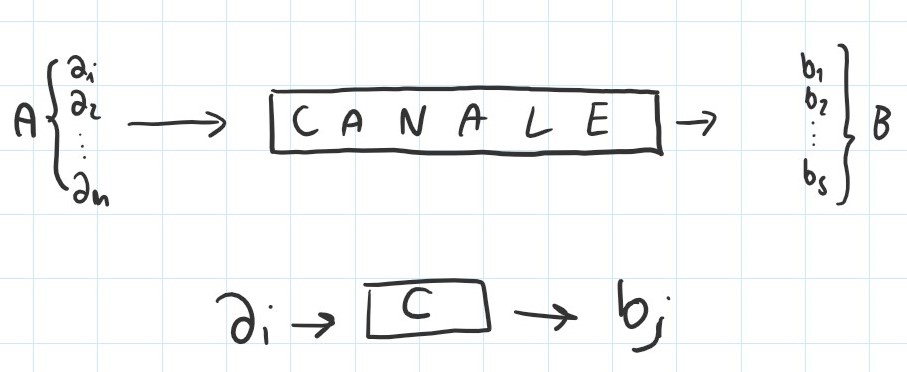
\includegraphics[width=0.8\linewidth]{immagini/img26}
\end{figure}
Esso è costituito da:
\begin{itemize}
	\item Simboli in input
	\item Simboli in output
	\item Probabilità condizionate
\end{itemize}
Ogni volta che inserisco un simbolo $a_i$ appartenente all'alfabeto $A$, il canale restituisce un simbolo $b_j$ appartenente all'alfabeto $B$.
Il rumore agisce sul simbolo $a_i$, facendo uscire un simbolo a seconda delle probabilità:
\begin{equation*}
P(b_j|a_i)
\end{equation*}
Per rappresentare tutte le probabilità condizionate uso una matrice di canale:

\begin{figure}[h]
	\centering
	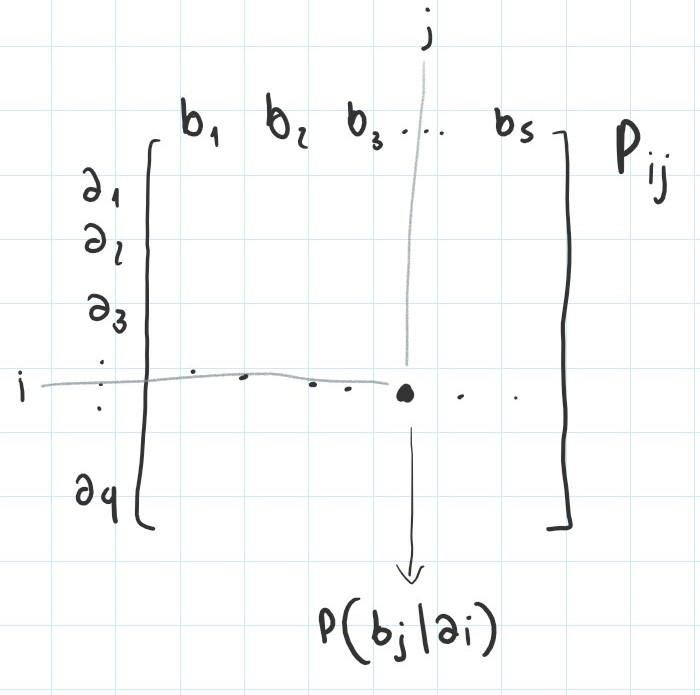
\includegraphics[width=0.57\linewidth]{immagini/img27}
\end{figure}

Quindi inserito un simbolo $a_i$ uscirà un simbolo $b$ in output basato sulle probabilità della riga $i$. Ovviamente dato un simbolo ne uscirà un altro sicuramente, quindi:
\begin{equation*}
\sum_{j=1}^sp(b_j|a_i)=\sum_{j=1}^sp_{ij} = 1
\end{equation*}
In altre parole ogni riga contiene una distribuzione discreta di probabilità, quindi la matrice è definita stocastica.

Se una riga ha tutti 0 e un 1 allora sappiamo che il simbolo su quella riga avrà sempre lo stesso simbolo in output (magari il canale è costruito in un certo modo, boh).

$p(a_i)$ è la probabilità con cui scegliamo il simbolo $a_i$ da inserire all'interno del canale. Quindi diciamo che l'utente inserisce nel canale il simbolo $a_i$ con questa probabilità.
Ci chiediamo quanto è la probabilità che esca $b_j$ (con $j=1,2,...s$).
Definiamo l'equazione di canale:
\begin{equation*}
p(b_j) =\sum_{i=1}^qp(b_j|a_i)p(a_i)
\end{equation*}
Quindi la probabilità di $b_j$ è la somma di più probabilità, in particolare ogni termine è la probabilità che esca $b_j$ dato che è stato inserito in ingresso $a_1$ oppure $a_2$ oppure $a_3$...
Il concetto viene più chiaro tramite questo grafo:
\begin{figure}[h]
	\centering
	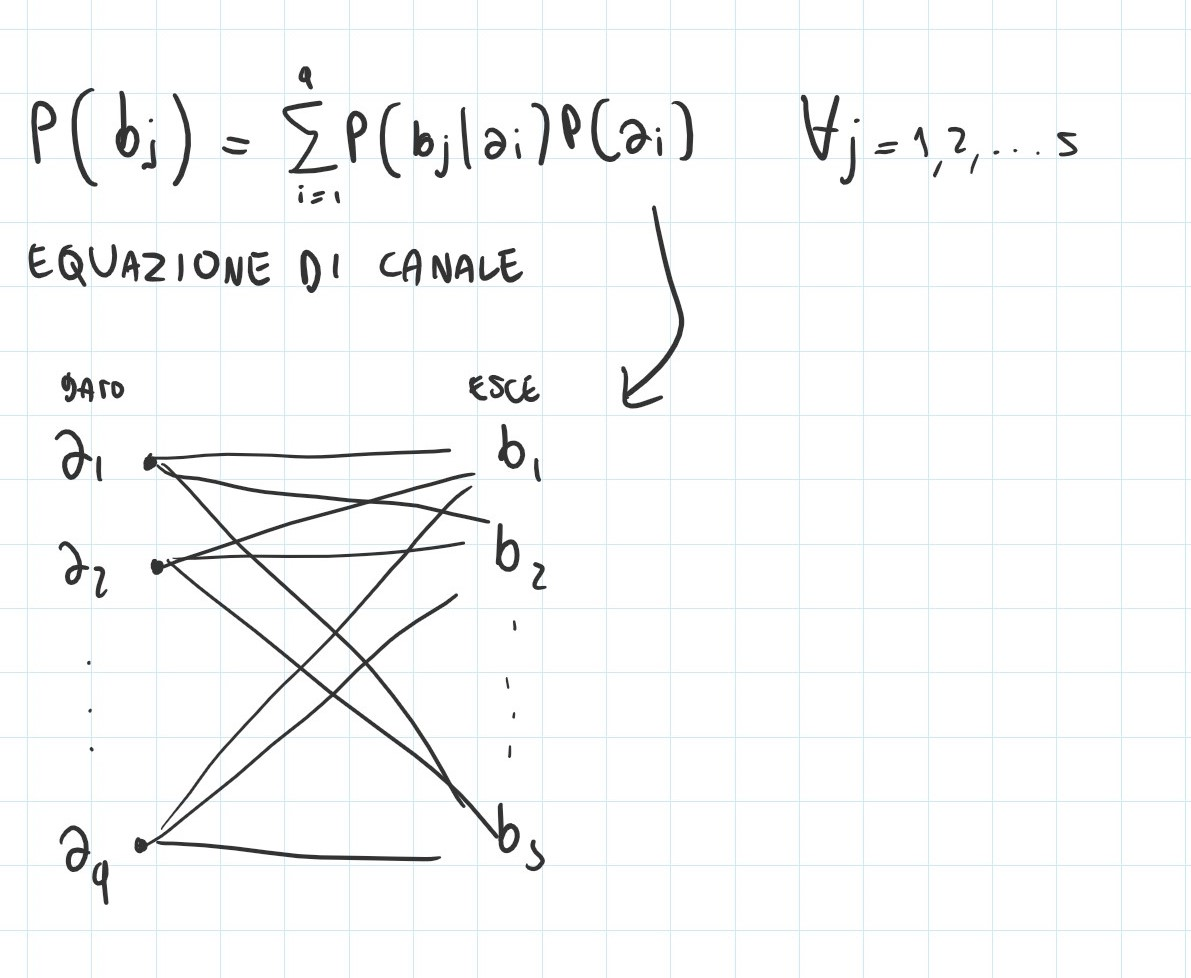
\includegraphics[width=0.85\linewidth]{immagini/img28}
\end{figure}

Vediamo ora due casi particolari (estremi, nella pratica non dovrebbero mai accadere):

\begin{itemize}
	\item Canale con assenza di rumore:\\
	Ogni volta che inserisco $a_i$ ho probabilità 1 che esca un certo $b_j$. Quindi la matrice di canale avrà tutte righe composte da 0 e 1.
	L'equazione di canale diventa:
	\begin{equation*}
	p(b_j) =\sum_{i=1}^qp(b_j|a_i)p(a_i) = 1 + 0 + ... + 0 = 1
	\end{equation*}
	\item Canale completamente rumoroso:\\
	Ogni simbolo inserito in input è completamente ignorato e l'output è totalmente casuale.
	In pratica le $b_j$ hanno una distribuzione di probabilità che dipende dal rumore e non da $a_i$.
	L'equazione di canale è:
	\begin{equation*}
	p(b_j) =\frac{1}{s} \; \; \; \; \forall j
	\end{equation*}
\end{itemize}

\subsection*{Probabilità condizionate all'indietro}
\addcontentsline{toc}{subsection}{Probabilità all'indietro}
Quando inserisco un simbolo in input $a_i$ sappiamo che la probabilità che esca $b_j$ è $p(b_j|a_i)$, ma quanto è la probabilità 'al contrario'? Ovvero, quanto è la probabilità che sia stato inviato $a_i$, visto che mi è arrivato $b_j$? Teorema di Bayes:
\begin{equation*}
p(a_i|b_j) = \frac{p(b_j|a_i)p(a_i)}{p(b_j)}
\end{equation*}
E usando l'equazione di canale:
\begin{equation*}
= \frac{p(b_j|a_i)p(a_i)}{\sum_{i=1}^qp(b_j|a_i)p(a_i)}
\end{equation*}
Consideriamo il canale più semplice (canale binario):
\begin{figure}[H]
	\centering
	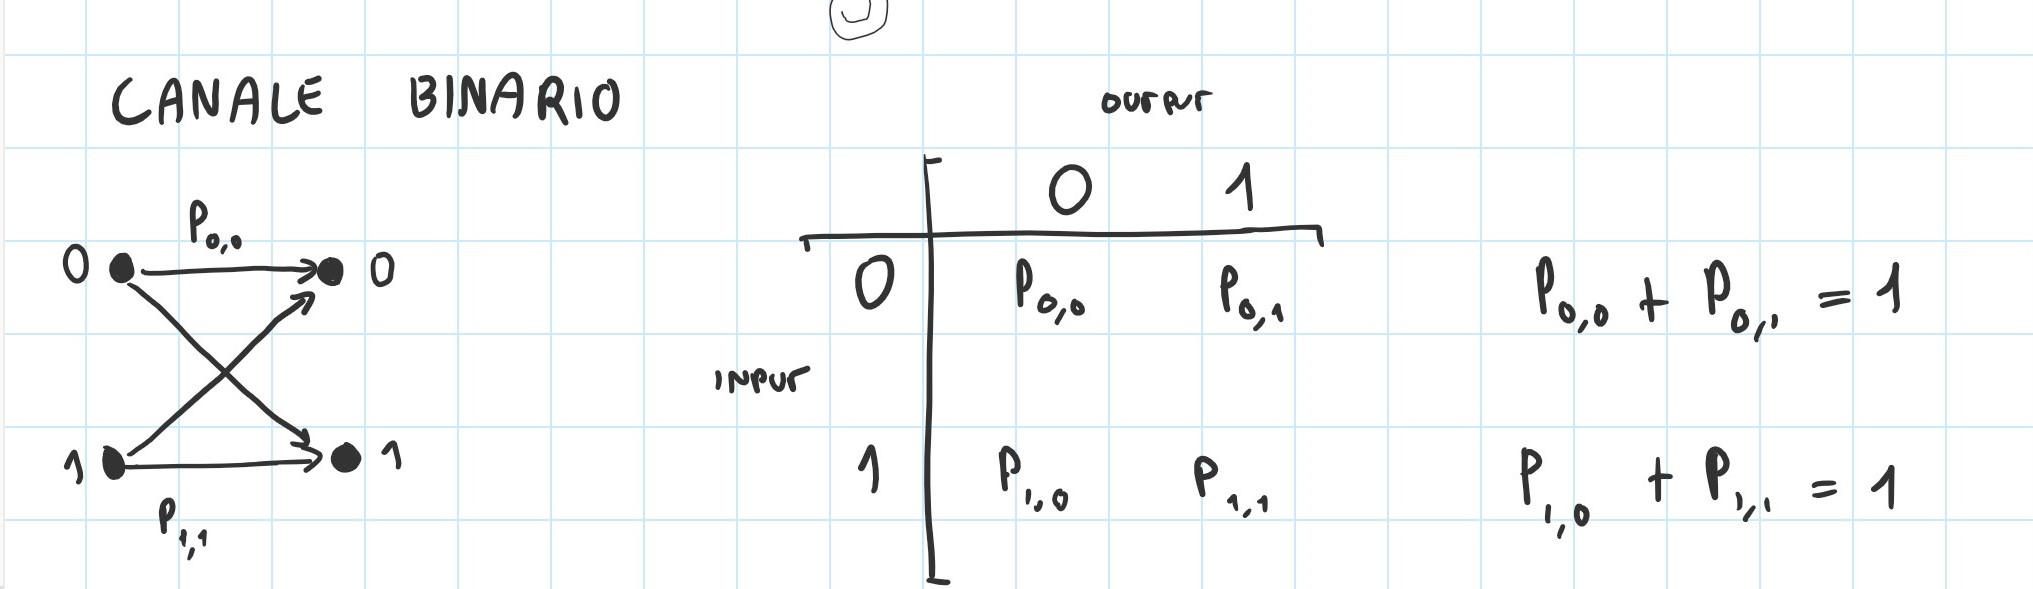
\includegraphics[width=\linewidth]{immagini/img29}
\end{figure}
La probabilità $p_{0,0} = p_{1,1}$ viene chiamata $P$, essa rappresenta la probabilità che inserito un bit dal canale esca lo stesso bit.
Chiamo $Q = 1-P$ la probabilità che la trasmissione sia errata.

La matrice di canale diventa:
\begin{equation*}
\begin{pmatrix}
P & Q\\
Q & P 
\end{pmatrix}
\end{equation*}

Questo tipo di canale è chiamato \textit{canale binario simmetrico} (CBS) in quanto la matrice che lo definisce è simmetrica.

Usando tanti canali CDS, voglio inviare un messaggio lungo $n$ bit, qual è la probabilità che il primo bit arrivi a destinazione sbagliato?\\
$Q$.\\
E che il secondo sbagli? $Q$. E così via.
I canali sono paralleli quindi gli eventi sono indipendenti (se uno sbaglia gli altri non vengono influenzati).
Questa descrizione è già stata vista: è il rumore bianco.
L'ennesima estensione della CDS ($\text{CDS}^n$) è il canale che rappresenta il rumore bianco.

Chiamo $a$ l'input del CDS e $b$ l'output. Chiamo inoltre $p$ la probabilità di scegliere $a=0$; $p(a=0)$.
Quindi $1-p$ è $p(a=1)$.
Chiamiamo $x$ la $p(b=0)$ e $1-x = p(b=1)$.
Le equazioni di canale ci dicono che:
\begin{equation*}
p(b=0) = pP + (1-p)Q
\end{equation*}
\begin{equation*}
p(b=1) = (1-p)P + pQ
\end{equation*}

Le probabilità all'indietro sono:

\begin{equation*}
p(a=0|b=0) = \frac{pP}{pP+(1-p)Q}
\end{equation*}


